\documentclass{beamer}
\usepackage[utf8]{inputenc}

\usepackage{utopia} %font utopia imported

\usepackage{biblatex}
\usepackage{ulem}           % packaged to strike out things
\usepackage{graphicx}
\graphicspath{{./img/}}

\addbibresource{references.bib}
\AtNextBibliography{\footnotesize}          % to make text smaller in bibliography
\setbeamertemplate{bibliography item}{}     % to remove images in bibliography


\usetheme{Berlin}
\usecolortheme{default}

%------------------------------------------------------------
%This block of code defines the information to appear in the
%Title page
\title[Approximate GPU] %optional
{Approximate GPU}

\subtitle{SoC-Lab WS19}

\author[David Freismuth (1326907), Andreas Glinserer (1525864), \\
Johannes Ivancsics (1325895)] % (optional)
{David Freismuth (1326907), Andreas Glinserer (1525864), Johannes Ivancsics (1325895)}

% \institute[VFU] % (optional)
% {
%   \inst{1}%
%   Faculty of Physics\\
%   Very Famous University
%   \and
%   \inst{2}%
%   Faculty of Chemistry\\
%   Very Famous University
% }

\date[\today] % (optional)
{\today}

%\logo{\includegraphics[height=1.5cm]{lion-logo.jpg}}

%End of title page configuration block
%------------------------------------------------------------



%------------------------------------------------------------
%The next block of commands puts the table of contents at the 
%beginning of each section and highlights the current section:

\AtBeginSection[]
{
  \begin{frame}
    \frametitle{Table of Contents}
    \tableofcontents[currentsection]
  \end{frame}
}
%------------------------------------------------------------


\begin{document}

%The next statement creates the title page.
\frame{\titlepage}


%---------------------------------------------------------
%This block of code is for the table of contents after
%the title page
\begin{frame}
\frametitle{Table of Contents}
\tableofcontents
\end{frame}
%---------------------------------------------------------

\section{Nyuzi GPU}
\begin{frame}{Nyuzi}
    \begin{itemize}
        \item<1-> Creator: Jeff Bush \cite{Nyuzi}
        \item<2-> Open Source (Verilog)
        \item<3-> Inspired by Intel's Larrabee \cite{Seiler:2008:LMX:1360612.1360617}
    \end{itemize}
\end{frame}
\begin{frame}{Block Diagram}
    \begin{figure}
        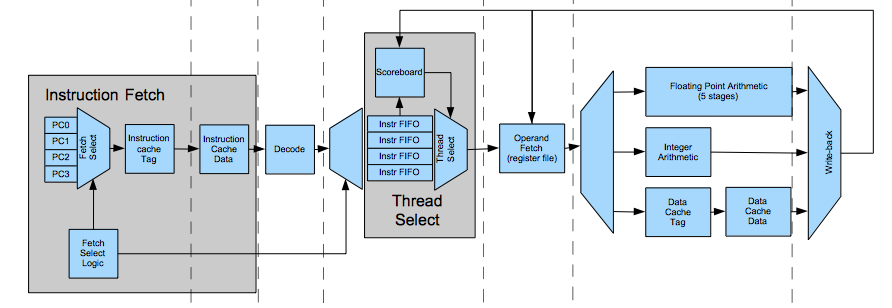
\includegraphics[width=\linewidth]{nyuzi-execute-pipeline}
        \caption{Execution Pipeline von Nyuzi}
    \end{figure}
\end{frame}

\begin{frame}{Floating Point Arithmetic}

% Stage	Addition	Multiplication
% 1	Compare exponents (and significands if exponents are equal). Use multiplexers to sort smaller and larger numbers into appropriate outputs.	Subtract exponents
% 2	Align smaller significand by shifting right. This stage collects guard, round, and sticky bits from the shifted out bits for rounding.	Multiply
% 3	Add/subtract (invert the significand for logical subtraction). Pre-normalization rounding occurs here based on GRS bits from above.	Multiply
% 4	Leading zero detection on significand for normalization.	Multiply
% 5	Normalize shift left. Post normalization rounding (only necessary for overflows).	Normalize/Round

\begin{table}[]
    \centering
    \begin{tabular}{l|l|l}
         Stage & Addition & Multiply \\ \hline \hline
         1 & Compare exponents & Subtract exponents \\
         2 & Align smaller exponent & Multiply\\
         3 & Add/Subtract & Multiply \\
         4 & Leading Zero detection & Multiply \\
         5 & Normalize Shift Left & Normalize/Round\\ \hline
    \end{tabular}
    \caption{Floating Point Stage}
    \label{tab:nyuzi_fpu}
\end{table}
    
\end{frame}

\begin{frame}{Challenges}
    \begin{itemize}
        \item<1-> SoC-Lab 2018 brought Nyuzi onto a FPGA\cite{NyuziKessler}
        \item<2-> Starting from there
        \item<3-> Doesn't compile anymore \ldots
    \end{itemize}
\end{frame}

%--------------------------------------------------------------------
\section{Approximation Techniques}

\begin{frame}{Targets}
\begin {columns}
 \begin{column}{0.7\textwidth}
 
    \begin{itemize}
        \item<1->Focus on \textit{"low hanging fruits"} described in \cite{Mittal:2016:STA:2891449.2893356}
        \item<2->Stay compatible to existing tool chain
        \item<3->Achieve a certain \textit{quality of result} (QoR)
        \item<4->Reduce area and power consumption
        \item<5->Only secondary: Throughput
    \end{itemize}
    
 \end{column}
  \begin{column}{0.3\textwidth}
    \begin{figure}
     
\includegraphics[width=\textwidth]{img/target.png}
     \caption{Source: https://tophatmedia.com.au/linkedin-done-for-you/png-photo-hd-target-0/}
    \end{figure}
  \end{column}
\end {columns}
\end{frame}

\begin{frame}{Precision Scaling}
\begin{columns}
\begin{column}{0.5\textwidth}
    \begin{itemize}
        \item<1->Lower the bit width of the functional units
        \item<2->Fewer logical gates are needed
            \begin{itemize}
                    \item<3-> Less area and power needed
                    \item<4-> Better timing higher achievable frequency
            \end{itemize}
        \item<5->May cause instability, if data dependency is high
    \end{itemize}
\end{column}
\begin{column}{0.5\textwidth}
    \begin{figure}
     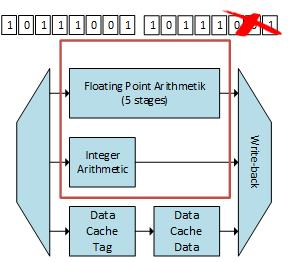
\includegraphics[width=\textwidth]{img/precisionReduction.jpg}
    \end{figure}

 \end{column}
\end{columns}
\end{frame}

\begin{frame}{Fixed Point Representation}
\begin {columns}
 \begin{column}{0.7\textwidth}
 
    \begin{itemize}
        \item<1->Remove floating point unit
        \item<2->Extend Integer unit to fixed point unit
        \item<3->No more pipeline $\rightarrow$ no more latency
        \item<4->Toolchain might have to be changed
    \end{itemize}
    
 \end{column}
  \begin{column}{0.3\textwidth}
    \begin{figure}
     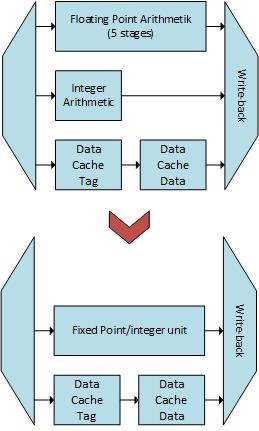
\includegraphics[width=\textwidth]{img/FixedPonitRepresentation.jpg}
     \caption{Source: https://tophatmedia.com.au/linkedin-done-for-you/png-photo-hd-target-0/}
    \end{figure}
  \end{column}
\end {columns}
\end{frame}

\begin{frame}{Inexact Hardware$^{\text{\cite{7974112}}}$}
\begin {columns}
 \begin{column}{0.7\textwidth}
 
    \begin{itemize}
        \item<1->Replace Adders/Multipliers with inexact combinatorial logic
        \item<2->Yields result within one clock cycle
        \item<3->Applicable to integer unit 
        \item<4->Applicable to mantisse operations
        \item<5->Reduces area and power consumption
        \item<6->No increase in Ops/second
    \end{itemize}
    
 \end{column}
  \begin{column}{0.3\textwidth}
    \begin{figure}
     
\includegraphics[width=\textwidth]{img/target.png}
     \caption{Source: https://tophatmedia.com.au/linkedin-done-for-you/png-photo-hd-target-0/}
    \end{figure}
  \end{column}
\end {columns}
\end{frame}

\begin{frame}{Load Value Approximation}
\begin {columns}
 \begin{column}{0.5\textwidth}
 
    \begin{itemize}
        \item<1->Estimate datum on cache miss
        \item<2->Avoid access to higher level memory $\rightarrow$ speed increase
        \item<3->Not viable in Nyuzi
        \item<4->Thread selector rearranges threads on cache miss
    \end{itemize}
    
 \end{column}
  \begin{column}{0.5\textwidth}
    \begin{figure}
     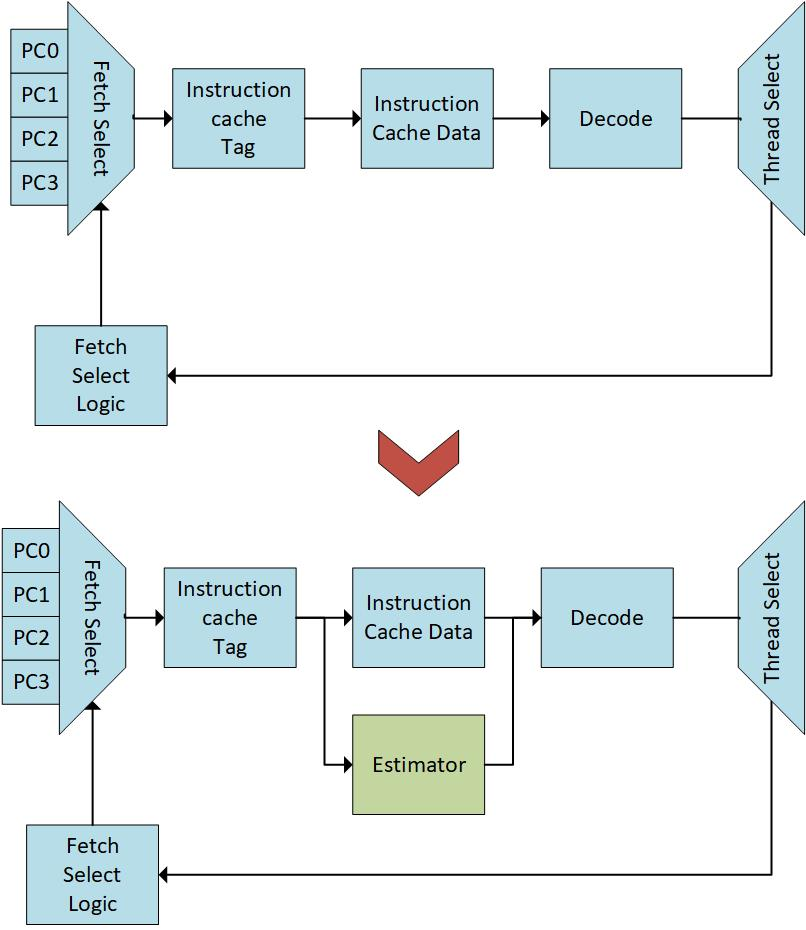
\includegraphics[width=\textwidth]{img/loadValueApproximation.jpg}
    \end{figure}
  \end{column}
\end {columns}
\end{frame}
%-------------------------------------------------------------------

\section{Evaluation}
\begin{frame}{Evaluation}
    \begin{itemize}
        \item<1-> Depends on application
        \item<2-> Balance quality loss $\leftrightarrow$ efficiency gain
        \item<3-> Quality of Result (QoR)
        \item<4-> Several metrics available
    \end{itemize}
\end{frame}

\begin{frame}{Evaluation areas}
    \begin{itemize}
        \item<1-> Focus on image processing
        \item<2-> Peak Signal-to-Noise Ratio (PSNR)
        \item<3-> Area consumption
        \item<4-> Power consumption
    \end{itemize}
\end{frame}

\begin{frame}{Use Doom for evaluation}
    \begin{itemize}
        \item<1-> Frames per second (FPS) analysis
        \item<2-> Instruction set simulator
        \item<3-> Reference value: 
            \begin{itemize}
                \item<1-> 8 FPS on i5 processor
                \item<2-> No optimisation for multithreading
                \item<3-> Does not use floating point unit
            \end{itemize}
    \end{itemize}
\end{frame}

\begin{frame}{Use Doom for evaluation}
    \begin{itemize}
        \item<1-> LIVE DEMONSTRATION 
    \end{itemize}    
\end{frame}

\section{Currently working on:}
\begin{frame}{}
    \begin{itemize}
        \item<1-> Evaluating the viable approaches
        \item<2-> Get existing work to work
    \end{itemize}
\end{frame}


\printbibliography




% \section{First section}


% %Changing visibility of the text
% \begin{frame}
% \frametitle{Sample frame title}
% This is a text in second frame. For the sake of showing an example.

% \begin{itemize}
%     \item<1-> Text visible on slide 1
%     \item<2-> Text visible on slide 2
%     \item<3> Text visible on slides 3
%     \item<4-> Text visible on slide 4
% \end{itemize}
% \end{frame}

% %---------------------------------------------------------


% %---------------------------------------------------------
% %Example of the \pause command
% \begin{frame}
% In this slide \pause

% the text will be partially visible \pause

% And finally everything will be there
% \end{frame}
% %---------------------------------------------------------

% \section{Second section}

% %---------------------------------------------------------
% %Highlighting text
% \begin{frame}
% \frametitle{Sample frame title}

% In this slide, some important text will be
% \alert{highlighted} because it's important.
% Please, don't abuse it.

% \begin{block}{Remark}
% Sample text
% \end{block}

% \begin{alertblock}{Important theorem}
% Sample text in red box
% \end{alertblock}

% \begin{examples}
% Sample text in green box. The title of the block is ``Examples".
% \end{examples}
% \end{frame}
% %---------------------------------------------------------


% %---------------------------------------------------------
% %Two columns
% \begin{frame}
% \frametitle{Two-column slide}

% \begin{columns}

% \column{0.5\textwidth}
% This is a text in first column.
% $$E=mc^2$$
% \begin{itemize}
% \item First item
% \item Second item
% \end{itemize}

% \column{0.5\textwidth}
% This text will be in the second column
% and on a second tought this is a nice looking
% layout in some cases.
% \end{columns}
% \end{frame}
% %---------------------------------------------------------


\end{document}



% Dieser Text ist urheberrechtlich geschützt
% Er stellt einen Auszug eines von mir erstellten Referates dar
% und darf nicht gewerblich genutzt werden
% die private bzw. Studiums bezogen Nutzung ist frei
% Mai. 2007
% Autor: Sascha Frank 
% Universität Freiburg 
% www.informatik.uni-freiburg.de/~frank/


% \documentclass{beamer}
% \setbeamertemplate{navigation symbols}{}
% \usepackage{beamerthemeshadow}
% \beamersetuncovermixins{\opaqueness<1>{25}}{\opaqueness<2->{15}}
% \begin{document}
% \title{Beamer Class ganz nett}  
% \author{Sascha Frank}
% \date{\today} 

% \begin{frame}
% \titlepage
% \end{frame} 

% \begin{frame}
% \frametitle{Inhaltsverzeichnis}\tableofcontents
% \end{frame} 


% \section{Abschnitt Nr.1} 
% \begin{frame}
% \frametitle{Titel} 
% Die einzelnen Frames sollte einen Titel haben 
% \end{frame}
% \subsection{Unterabschnitt Nr.1.1  }
% \begin{frame} 
% Denn ohne Titel fehlt ihnen was
% \end{frame}


% \section{Abschnitt Nr. 2} 
% \subsection{Listen I}
% \begin{frame}\frametitle{Aufz\"ahlung}
% \begin{itemize}
% \item Einf\"uhrungskurs in \LaTeX  
% \item Kurs 2  
% \item Seminararbeiten und Pr\"asentationen mit \LaTeX 
% \item Die Beamerclass 
% \end{itemize} 
% \end{frame}

% \begin{frame}\frametitle{Aufz\"ahlung mit Pausen}
% \begin{itemize}
% \item  Einf\"uhrungskurs in \LaTeX \pause 
% \item  Kurs 2 \pause 
% \item  Seminararbeiten und Pr\"asentationen mit \LaTeX \pause 
% \item  Die Beamerclass
% \end{itemize} 
% \end{frame}

% \subsection{Listen II}
% \begin{frame}\frametitle{Numerierte Liste}
% \begin{enumerate}
% \item  Einf\"uhrungskurs in \LaTeX 
% \item  Kurs 2
% \item  Seminararbeiten und Pr\"asentationen mit \LaTeX 
% \item  Die Beamerclass
% \end{enumerate}
% \end{frame}
% \begin{frame}\frametitle{Numerierte Liste mit Pausen}
% \begin{enumerate}
% \item  Einf\"uhrungskurs in \LaTeX \pause 
% \item  Kurs 2 \pause 
% \item  Seminararbeiten und Pr\"asentationen mit \LaTeX \pause 
% \item  Die Beamerclass
% \end{enumerate}
% \end{frame}

% \section{Abschnitt Nr.3} 
% \subsection{Tabellen}
% \begin{frame}\frametitle{Tabellen}
% \begin{tabular}{|c|c|c|}
% \hline
% \textbf{Zeitpunkt} & \textbf{Kursleiter} & \textbf{Titel} \\
% \hline
% WS 04/05 & Sascha Frank &  Erste Schritte mit \LaTeX  \\
% \hline
% SS 05 & Sascha Frank & \LaTeX \ Kursreihe \\
% \hline
% \end{tabular}
% \end{frame}


% \begin{frame}\frametitle{Tabellen mit Pause}
% \begin{tabular}{c c c}
% A & B & C \\ 
% \pause 
% 1 & 2 & 3 \\  
% \pause 
% A & B & C \\ 
% \end{tabular} 
% \end{frame}


% \section{Abschnitt Nr. 4}
% \subsection{Bl\"ocke}
% \begin{frame}\frametitle{Bl\"ocke}

% \begin{block}{Blocktitel}
% Blocktext 
% \end{block}

% \begin{exampleblock}{Blocktitel}
% Blocktext 
% \end{exampleblock}


% \begin{alertblock}{Blocktitel}
% Blocktext 
% \end{alertblock}
% \end{frame}

% \section{Abschnitt Nr. 5}
% \subsection{Geteilter Bildschirm}

% \begin{frame}\frametitle{Zerteilen des Bildschirmes}
% \begin{columns}
% \begin{column}{5cm}
% \begin{itemize}
% \item Beamer 
% \item Beamer Class 
% \item Beamer Class Latex 
% \end{itemize}
% \end{column}
% \begin{column}{5cm}
% \begin{tabular}{|c|c|}
% \hline
% \textbf{Kursleiter} & \textbf{Titel} \\
% \hline
% Sascha Frank &  \LaTeX \ Kurs 1 \\
% \hline
% Sascha Frank & \LaTeX \ Kursreihe \\
% \hline
% \end{tabular}
% \end{column}
% \end{columns}
% \end{frame}

% \subsection{Bilder} 
% \begin{frame}\frametitle{Bilder in Beamer}
% \begin{figure}
% \includegraphics[scale=0.5]{PIC1} 
% \caption{Die Abbildung zeigt ein Beispielbild}
% \end{figure}
% \end{frame}


% \subsection{Bilder und Listen kombiniert} 

% \begin{frame}
% \frametitle{Bilder und Itemization in Beamer}
% \begin{columns}
% \begin{column}{5cm}
% \begin{itemize}
% \item<1-> Stichwort 1
% \item<3-> Stichwort 2
% \item<5-> Stichwort 3
% \end{itemize}
% \vspace{3cm} 
% \end{column}
% \begin{column}{5cm}
% \begin{overprint}
% \includegraphics<2>{PIC1}
% \includegraphics<4>{PIC2}
% \includegraphics<6>{PIC3}
% \end{overprint}
% \end{column}
% \end{columns}
% \end{frame}

% \subsection{Bilder die mehr Platz brauchen} 
% \begin{frame}[plain]
% \frametitle{plain, oder wie man mehr Platz hat}
% \begin{figure}
% \includegraphics[scale=0.5]{PIC1} 
% \caption{Die Abbildung zeigt ein Beispielbild}
% \end{figure}
% \end{frame}
